
\documentclass[11pt,a4paper]{article}
\usepackage[T1]{fontenc}
\usepackage{lmodern}
\usepackage{amsmath,amssymb,amsfonts,mathtools}
\usepackage{graphicx,booktabs,longtable,array,tabularx,adjustbox}
\usepackage{geometry,microtype,fancyhdr,lastpage,etoolbox,enumitem}
\usepackage{newunicodechar,textcomp}
\usepackage{hyperref}
\hypersetup{hidelinks,pdfcreator={XeLaTeX / QM1 academic edition}}
\geometry{left=20mm,right=20mm,top=22mm,bottom=23mm}
\setcounter{secnumdepth}{2}
\setlength{\parindent}{0pt}
\setlength{\parskip}{4pt plus 1pt}
\setlength{\emergencystretch}{2em}
\setlength{\tabcolsep}{3pt}
\renewcommand{\arraystretch}{1.16}
\setlist{nosep,topsep=3pt,itemsep=2pt,leftmargin=7mm}
\AtBeginEnvironment{longtable}{\footnotesize\setlength{\tabcolsep}{2.2pt}}
\newcommand{\tightlist}{\setlength{\itemsep}{0pt}\setlength{\parskip}{0pt}}
\providecommand{\Cov}{\operatorname{Cov}}
\providecommand{\Var}{\operatorname{Var}}
\providecommand{\Corr}{\operatorname{Corr}}
\providecommand{\MAD}{\operatorname{MAD}}
\providecommand{\E}{\mathbb{E}}
\providecommand{\R}{\mathbb{R}}
\newunicodechar{—}{\textemdash}
\newunicodechar{–}{\textendash}
\newunicodechar{€}{\texteuro}
\newunicodechar{≤}{\ensuremath{\leq}}
\newunicodechar{≥}{\ensuremath{\geq}}
\newunicodechar{×}{\ensuremath{\times}}
\newunicodechar{÷}{\ensuremath{\div}}
\newunicodechar{Σ}{\ensuremath{\Sigma}}
\newunicodechar{σ}{\ensuremath{\sigma}}
\newunicodechar{μ}{\ensuremath{\mu}}
\newunicodechar{Δ}{\ensuremath{\Delta}}
\newunicodechar{∑}{\ensuremath{\sum}}
\newunicodechar{≈}{\ensuremath{\approx}}
\newunicodechar{√}{\ensuremath{\surd}}
\newunicodechar{≠}{\ensuremath{\ne}}
\newunicodechar{→}{\ensuremath{\to}}
\newunicodechar{∞}{\ensuremath{\infty}}
\newunicodechar{∈}{\ensuremath{\in}}
\newunicodechar{−}{\ensuremath{-}}
\newunicodechar{²}{\ensuremath{^{2}}}
\newunicodechar{³}{\ensuremath{^{3}}}
\newunicodechar{₀}{\ensuremath{_{0}}}
\newunicodechar{₁}{\ensuremath{_{1}}}
\newunicodechar{₂}{\ensuremath{_{2}}}
\newunicodechar{₃}{\ensuremath{_{3}}}
\newunicodechar{₄}{\ensuremath{_{4}}}
\newunicodechar{ₜ}{\ensuremath{_{t}}}
\newunicodechar{ₚ}{\ensuremath{_{p}}}
\newunicodechar{ₙ}{\ensuremath{_{n}}}
\newunicodechar{ₓ}{\ensuremath{_{x}}}
\newunicodechar{ᵢ}{\ensuremath{_{i}}}
\newunicodechar{ŷ}{\ensuremath{\hat y}}
\newunicodechar{Ŷ}{\ensuremath{\widehat Y}}
\newunicodechar{ₘ}{\ensuremath{_{m}}}
\newunicodechar{ₑ}{\ensuremath{_{e}}}
\newunicodechar{ₐ}{\ensuremath{_{a}}}
\newunicodechar{ₖ}{\ensuremath{_{k}}}
\newunicodechar{ₛ}{\ensuremath{_{s}}}
\newunicodechar{ₗ}{\ensuremath{_{l}}}
\newunicodechar{ₕ}{\ensuremath{_{h}}}
\newunicodechar{ₒ}{\ensuremath{_{o}}}
\newunicodechar{₊}{\ensuremath{_{+}}}
\newunicodechar{₋}{\ensuremath{_{-}}}
\newunicodechar{₌}{\ensuremath{_{=}}}
\newunicodechar{₍}{\ensuremath{_{(}}}
\newunicodechar{₎}{\ensuremath{_{)}}}
\newunicodechar{⁻}{\ensuremath{^{-}}}
\newunicodechar{⁺}{\ensuremath{^{+}}}
\newunicodechar{⁰}{\ensuremath{^{0}}}
\newunicodechar{¹}{\ensuremath{^{1}}}
\newunicodechar{⁴}{\ensuremath{^{4}}}
\newunicodechar{⁵}{\ensuremath{^{5}}}
\newunicodechar{⁶}{\ensuremath{^{6}}}
\newunicodechar{⁷}{\ensuremath{^{7}}}
\newunicodechar{⁸}{\ensuremath{^{8}}}
\newunicodechar{⁹}{\ensuremath{^{9}}}
\makeatletter
\renewcommand{\section}{\@startsection{section}{1}{0pt}{2.0ex plus .7ex minus .3ex}{1.0ex}{\large\bfseries}}
\renewcommand{\subsection}{\@startsection{subsection}{2}{0pt}{1.8ex plus .5ex minus .2ex}{.7ex}{\normalsize\bfseries}}
\renewcommand{\subsubsection}{\@startsection{subsubsection}{3}{0pt}{1.3ex plus .4ex minus .2ex}{.5ex}{\normalsize\bfseries}}
\makeatother
\pagestyle{fancy}
\fancyhf{}
\renewcommand{\headrulewidth}{0.35pt}
\renewcommand{\footrulewidth}{0pt}
\fancyhead[L]{\small\textsc{KEDGE Business School --- QM1}}
\fancyhead[R]{\small\textsc{2026--2027}}
\fancyfoot[L]{\small Badr ABOUFARASSE, PhD}
\fancyfoot[R]{\small\thepage\ /\ \pageref{LastPage}}
\setlength{\headheight}{14pt}
\setkeys{Gin}{keepaspectratio}
\begin{document}

\begin{center}
{\small\textsc{KEDGE Business School \quad EBP1 \quad Quantitative Methods 1}}\\[6pt]
{\Large\bfseries Fiche 3 — Dispersion et concentration}\\[6pt]
{\normalsize\bfseries Corrigés intégralement détaillés}\\[6pt]
{\small Badr ABOUFARASSE, PhD \quad --- \quad 2026--2027}
\end{center}
\vspace{2mm}\hrule\vspace{6mm}

\hypertarget{applications-fondamentales}{%
\section{Applications fondamentales}\label{applications-fondamentales}}

Maîtriser les définitions et les calculs essentiels du cours.

\emph{Application du cours --- 25 min}

\hypertarget{exercice-4-muxe9diale-et-masses-relatives}{%
\subsection{Exercice 4 --- Médiale et masses relatives}\label{exercice-4-muxe9diale-et-masses-relatives}}

On observe la dépense (en €) de 40 clients. Approcher la masse monétaire de chaque classe par nᵢ × centre de classe.

\begin{longtable}[]{@{}llllll@{}}
\toprule\noalign{}
Classe / Class & {[}10,20{[} & {[}20,30{[} & {[}30,40{[} & {[}40,50{[} & {[}50,60{[} \\
\midrule\noalign{}
\endhead
\bottomrule\noalign{}
\endlastfoot
nᵢ & 8 & 12 & 10 & 6 & 4 \\
\end{longtable}

\begin{enumerate}
\tightlist
\item
  Calculer les centres, masses, masses cumulées et parts relatives cumulées.
\item
  Calculer la médiale par interpolation dans la classe contenant 50 \% de la masse.
\item
  Calculer la médiane des effectifs et comparer les deux mesures.
\end{enumerate}

\hypertarget{corriguxe9-duxe9tailluxe9}{%
\subsubsection{Corrigé détaillé}\label{corriguxe9-duxe9tailluxe9}}

\begin{longtable}[]{@{}llllll@{}}
\toprule\noalign{}
Classe / Class & nᵢ & cᵢ & nᵢcᵢ & Masse cumulée & Masse cumulée (\%) \\
\midrule\noalign{}
\endhead
\bottomrule\noalign{}
\endlastfoot
{[}10,20{[} & 8 & 15 & 120 & 120 & 9.52 \\
{[}20,30{[} & 12 & 25 & 300 & 420 & 33.33 \\
{[}30,40{[} & 10 & 35 & 350 & 770 & 61.11 \\
{[}40,50{[} & 6 & 45 & 270 & 1040 & 82.54 \\
{[}50,60{[} & 4 & 55 & 220 & 1260 & 100 \\
TOTAL & 40 & --- & 1260 & --- & 100 \\
\end{longtable}

\[S=\sum n_ic_i=120+300+350+270+220=1260,\qquad S/2=630.\]

La moitié de la masse se trouve dans {[}30,40{[}, car 420 \textless{} 630 ≤ 770. Sous l\textquotesingle hypothèse d\textquotesingle interpolation linéaire de la masse :

\[MI=30+\frac{630-420}{350}\times10=36\ \mathrm{euros}.\]

La médiane des effectifs est 30 € (20 observations sur 40 avant 30 €). La médiale, 36 €, partage la masse monétaire et non les effectifs.

\emph{Application du cours --- 20 min}

\hypertarget{compluxe9ment-1-dispersion-uxe0-partir-dun-tableau-de-fruxe9quences}{%
\subsection{Complément 1 --- Dispersion à partir d'un tableau de fréquences}\label{compluxe9ment-1-dispersion-uxe0-partir-dun-tableau-de-fruxe9quences}}

Le nombre de réclamations hebdomadaires par magasin est distribué ainsi :

\begin{longtable}[]{@{}llllll@{}}
\toprule\noalign{}
Réclamations x & 0 & 1 & 2 & 3 & 4 \\
\midrule\noalign{}
\endhead
\bottomrule\noalign{}
\endlastfoot
Magasins n & 4 & 8 & 10 & 6 & 2 \\
\end{longtable}

\begin{enumerate}
\tightlist
\item
  Calculez la moyenne, la variance de population et l'écart-type.
\item
  Calculez le coefficient de variation.
\item
  Interprétez chaque résultat.
\end{enumerate}

\textbf{Indication méthodologique :}

Construisez les colonnes nx et nx². Utilisez E(X²) − {[}E(X){]}² pour la variance de population.

\hypertarget{corriguxe9-duxe9tailluxe9-1}{%
\subsubsection{Corrigé détaillé}\label{corriguxe9-duxe9tailluxe9-1}}

\textbf{Totaux.} N = 30 ; Σnx = 54 ; Σnx² = 134.

\textbf{Moyenne.} 54/30 = \textbf{1,80 réclamation}.

\textbf{Variance.} E(X²) = 134/30 = 4,4667 ; σ² = 4,4667 − 1,80² = \textbf{1,2267}.

\textbf{Écart-type.} σ = √1,2267 = \textbf{1,108 réclamation}.

\textbf{Coefficient de variation.} CV = 1,108/1,80 × 100 = \textbf{61,6 \%}.

\textbf{Interprétation.} Les magasins enregistrent en moyenne 1,8 réclamation, avec une forte hétérogénéité relative. La comparaison suppose la même période et la même définition d'une réclamation.

\begin{longtable}[]{@{}llll@{}}
\toprule\noalign{}
xᵢ & nᵢ & nᵢxᵢ & nᵢxᵢ² \\
\midrule\noalign{}
\endhead
\bottomrule\noalign{}
\endlastfoot
0 & 4 & 0 & 0 \\
1 & 8 & 8 & 8 \\
2 & 10 & 20 & 40 \\
3 & 6 & 18 & 54 \\
4 & 2 & 8 & 32 \\
Σ & 30 & 54 & 134 \\
\end{longtable}

\hypertarget{pruxe9paration-aux-uxe9valuations}{%
\section{Préparation aux évaluations}\label{pruxe9paration-aux-uxe9valuations}}

Résoudre des exercices de contrôle continu et de partiel en autonomie.

\emph{Préparation CC / partiel --- 35 min}

\hypertarget{exercice-2-dispersion-dune-distribution-groupuxe9e}{%
\subsection{Exercice 2 -- Dispersion d'une distribution groupée}\label{exercice-2-dispersion-dune-distribution-groupuxe9e}}

Reprendre la distribution des 210 clients de la fiche 2. À partir des centres de classes :

\begin{enumerate}
\item
  calculer {\(\sum n_ic_i\)} et {\(\sum n_ic_i^2\)} ;
\item
  calculer la moyenne, la variance de population et l'écart-type ;
\item
  calculer le coefficient de variation ;
\item
  calculer l'écart interquartile ;
\item
  comparer l'information fournie par l'écart-type et par l'IQR.
\end{enumerate}

\hypertarget{corriguxe9-duxe9tailluxe9-2}{%
\subsubsection{Corrigé détaillé}\label{corriguxe9-duxe9tailluxe9-2}}

À partir des centres : {\[\sum n_ic_i=6665,
\qquad
\sum n_ic_i^2=227036.5.\]} {\[\bar
x=\frac{6665}{210}\approx31.7381.\]} {\[V=\frac{227036.5}{210}-\bar
x^2\approx73.8195.\]} {\[\sigma=\sqrt{73.8195}\approx8.5918.\]} {\[CV=\frac{8.5918}{31.7381}\approx0.2707=27.07\%.\]} Avec {\(Q_1\approx26.56\)} et {\(Q_3=37.50\)} : {\[IQR=37.50-26.56\approx10.94.\]} L'écart-type utilise toutes les observations et est sensible aux extrêmes. L'IQR décrit la dispersion de la moitié centrale et est plus robuste aux valeurs extrêmes.

\hypertarget{duxe9tail-des-produits-ponduxe9ruxe9s}{%
\subsubsection{Détail des produits pondérés}\label{duxe9tail-des-produits-ponduxe9ruxe9s}}

\begin{longtable}[]{@{}lllll@{}}
\toprule\noalign{}
Classe & n & c & n×c & n×c² \\
\midrule\noalign{}
\endhead
\bottomrule\noalign{}
\endlastfoot
{[}10,14{[} & 4 & 12 & 48 & 576.00 \\
{[}14,18{[} & 12 & 16 & 192 & 3072.00 \\
{[}18,26{[} & 32 & 22 & 704 & 15488.00 \\
{[}26,30{[} & 32 & 28 & 896 & 25088.00 \\
{[}30,35{[} & 60 & 32.5 & 1950 & 63375.00 \\
{[}35,40{[} & 35 & 37.5 & 1312.5 & 49218.75 \\
{[}40,45{[} & 25 & 42.5 & 1062.5 & 45156.25 \\
{[}45,50{[} & 5 & 47.5 & 237.5 & 11281.25 \\
{[}50,55{[} & 5 & 52.5 & 262.5 & 13781.25 \\
Σ & 210 & --- & 6665 & 227036.50 \\
\end{longtable}

\[\begin{gathered}
V=\frac{227036.5}{210}-\left(\frac{6665}{210}\right)^2=73.8195,\\\sigma=\sqrt{73.8195}=8.5918.
\end{gathered}\]

La variance calculée à partir des centres est une approximation de la dispersion des observations individuelles.

\emph{Préparation CC / partiel --- 30 min}

\hypertarget{exercice-3-courbe-de-lorenz-et-indice-de-gini}{%
\subsection{Exercice 3 -- Courbe de Lorenz et indice de Gini}\label{exercice-3-courbe-de-lorenz-et-indice-de-gini}}

Cinq revenus, déjà classés par ordre croissant, valent : {\[10,\ 12,\ 18,\ 25,\ 35.\]}

\begin{enumerate}
\item
  Calculer le revenu total et les parts cumulées de population et de revenu.
\item
  Construire la courbe de Lorenz.
\item
  Calculer l'aire sous la courbe par la méthode des trapèzes.
\item
  En déduire le coefficient de Gini et l'interpréter.
\item
  Expliquer pourquoi le Gini décrit la concentration sans expliquer ses causes.
\end{enumerate}

\hypertarget{corriguxe9-duxe9tailluxe9-3}{%
\subsubsection{Corrigé détaillé}\label{corriguxe9-duxe9tailluxe9-3}}

Revenu total : {\[10+12+18+25+35=100.\]} Les points de Lorenz sont : {\[(0,0),\ (0.2,0.10),\ (0.4,0.22),\
(0.6,0.40),\ (0.8,0.65),\ (1,1).\]} Aire sous la courbe par trapèzes : {\[A=0.2\left(\frac{0+0.10}{2}+\frac{0.10+0.22}{2}+\frac{0.22+0.40}{2}+\frac{0.40+0.65}{2}+\frac{0.65+1}{2}\right).\]} {\[A=0.374.\]} Donc : {\[G=1-2A=1-0.748=0.252=25.2\%.\]}

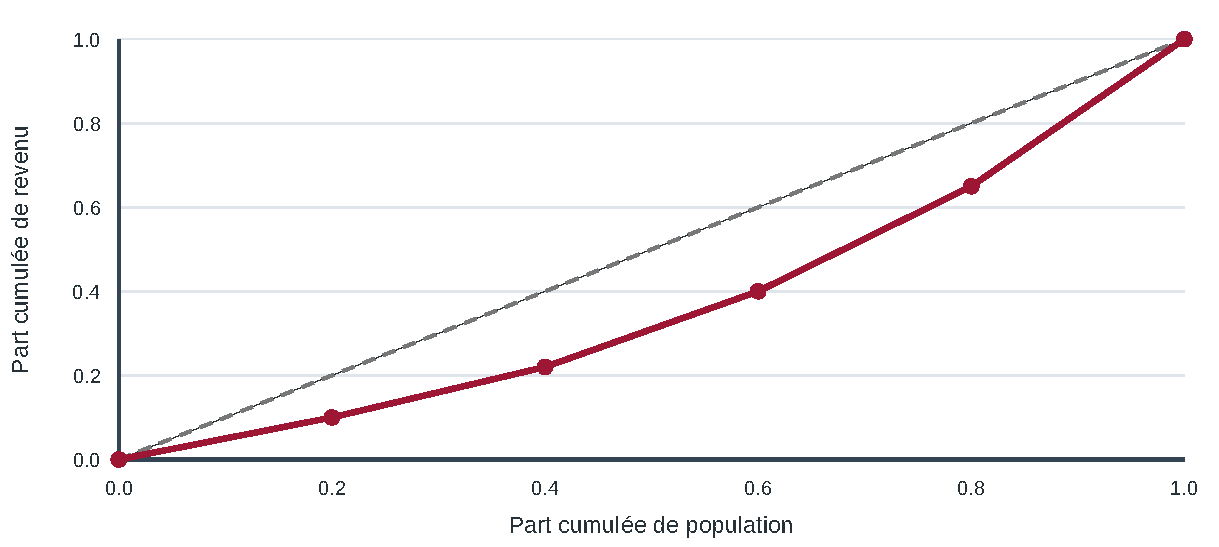
\includegraphics[width=0.85\textwidth,height=\textheight]{assets/chapter-3-solutions-fr-chart-01.pdf}

\emph{Courbe de Lorenz et ligne d'égalité}

Le Gini résume le degré de concentration, mais il ne permet pas d'identifier les mécanismes économiques ou institutionnels à l'origine de cette concentration.

\hypertarget{approfondissement-facultatif}{%
\section{Approfondissement facultatif}\label{approfondissement-facultatif}}

Aller plus loin dans l'interprétation et les applications professionnelles.

\emph{Approfondissement --- 30 min}

\hypertarget{exercice-1-boxplot-valeurs-atypiques-et-choix-de-la-variance}{%
\subsection{Exercice 1 -- Boxplot, valeurs atypiques et choix de la variance}\label{exercice-1-boxplot-valeurs-atypiques-et-choix-de-la-variance}}

On observe : {\[5,6,6,7,7,8,8,9,9,10,11,20.\]} On utilisera la convention « médiane des moitiés » pour les quartiles.

\begin{enumerate}
\item
  Calculer le résumé à cinq nombres : minimum, {\(Q_1\)}, médiane, {\(Q_3\)}, maximum.
\item
  Calculer l'étendue et l'écart interquartile {\(IQR\)}.
\item
  Calculer les bornes {\(Q_1-1.5IQR\)} et {\(Q_3+1.5IQR\)} et identifier les valeurs atypiques potentielles.
\item
  Calculer la moyenne et l'écart absolu moyen.
\item
  Calculer la variance et l'écart-type si ces 12 observations constituent toute la population.
\item
  Calculer la variance et l'écart-type corrigés si elles constituent un échantillon.
\end{enumerate}

\hypertarget{corriguxe9-duxe9tailluxe9-4}{%
\subsubsection{Corrigé détaillé}\label{corriguxe9-duxe9tailluxe9-4}}

Données ordonnées : {\(5,6,6,7,7,8,8,9,9,10,11,20\)}. {\[\min=5,\qquad Me=\frac{8+8}{2}=8,\qquad
\max=20.\]} Moitié basse : {\(5,6,6,7,7,8\)}, donc {\[Q_1=\frac{6+7}{2}=6.5.\]} Moitié haute : {\(8,9,9,10,11,20\)}, donc {\[Q_3=\frac{9+10}{2}=9.5.\]} Ainsi : {\[IQR=Q_3-Q_1=9.5-6.5=3.\]} Les bornes sont : {\[B_{\inf}=6.5-1.5(3)=2,
\qquad
B_{\sup}=9.5+1.5(3)=14.\]} Comme {\(20>14\)}, la valeur 20 est une valeur atypique potentielle.

Somme des valeurs : {\(106\)}, donc : {\[\bar
x=\frac{106}{12}\approx8.8333.\]} L'écart absolu moyen vaut : {\[e=\frac{1}{12}\sum_{i=1}^{12}|x_i-\bar
x|\approx2.4722.\]} Variance de population : {\[\sigma^2=\frac{1}{12}\sum_{i=1}^{12}(x_i-\bar
x)^2\approx14.1389,\]} {\[\sigma\approx3.7602.\]} Variance d'échantillon : {\[s^2=\frac{1}{11}\sum_{i=1}^{12}(x_i-\bar
x)^2\approx15.4242,\]} {\[s\approx3.9274.\]}

\hypertarget{tableau-de-tous-les-uxe9carts}{%
\subsubsection{Tableau de tous les écarts}\label{tableau-de-tous-les-uxe9carts}}

\begin{longtable}[]{@{}llll@{}}
\toprule\noalign{}
i & x & \textbar x−106/12\textbar{} & (x−106/12)² \\
\midrule\noalign{}
\endhead
\bottomrule\noalign{}
\endlastfoot
1 & 5 & 3.8333 & 14.6944 \\
2 & 6 & 2.8333 & 8.0278 \\
3 & 6 & 2.8333 & 8.0278 \\
4 & 7 & 1.8333 & 3.3611 \\
5 & 7 & 1.8333 & 3.3611 \\
6 & 8 & 0.8333 & 0.6944 \\
7 & 8 & 0.8333 & 0.6944 \\
8 & 9 & 0.1667 & 0.0278 \\
9 & 9 & 0.1667 & 0.0278 \\
10 & 10 & 1.1667 & 1.3611 \\
11 & 11 & 2.1667 & 4.6944 \\
12 & 20 & 11.1667 & 124.6944 \\
Σ & 106 & 29.6667 & 169.6667 \\
\end{longtable}

\[\sum x_i^2=1106,\quad\sum(x_i-\bar x)^2=1106-\frac{106^2}{12}=169.6667.\]

\[e=29.6667/12=2.4722,\quad \sigma^2=169.6667/12=14.1389,\quad s^2=169.6667/11=15.4242.\]

Les valeurs du tableau sont arrondies pour l'affichage : calculer avec les fractions exactes avant l'arrondi final.

\emph{Approfondissement --- 25 min}

\hypertarget{compluxe9ment-2-comparer-concentration-et-robustesse}{%
\subsection{Complément 2 --- Comparer concentration et robustesse}\label{compluxe9ment-2-comparer-concentration-et-robustesse}}

Deux marchés présentent les parts de marché ordonnées suivantes :

\begin{longtable}[]{@{}llllll@{}}
\toprule\noalign{}
Marché A & 10 \% & 15 \% & 20 \% & 25 \% & 30 \% \\
Marché B & 2 \% & 8 \% & 10 \% & 20 \% & 60 \% \\
\midrule\noalign{}
\endhead
\bottomrule\noalign{}
\endlastfoot
\end{longtable}

\begin{enumerate}
\tightlist
\item
  Construisez les parts cumulées.
\item
  Indiquez quelle courbe de Lorenz est la plus éloignée de l'égalité.
\item
  Calculez les étendues et expliquez leur limite.
\item
  Formulez une conclusion défendable.
\end{enumerate}

\textbf{Indication méthodologique :}

Avec cinq entreprises de même poids, les parts cumulées de population progressent de 20 points.

\hypertarget{corriguxe9-duxe9tailluxe9-5}{%
\subsubsection{Corrigé détaillé}\label{corriguxe9-duxe9tailluxe9-5}}

\textbf{Parts cumulées.} Marché A : 0 \%, 10 \%, 25 \%, 45 \%, 70 \%, 100 \%. Marché B : 0 \%, 2 \%, 10 \%, 20 \%, 40 \%, 100 \%. Les parts de population sont 0 \%, 20 \%, 40 \%, 60 \%, 80 \%, 100 \%.

\textbf{Lorenz.} À chaque point intérieur, la part cumulée de B est plus faible : sa courbe est plus éloignée de l'égalité et la concentration plus forte.

\textbf{Étendues.} A : 30−10 = 20 points ; B : 60−2 = 58 points. L'étendue confirme l'écart, mais n'utilise que les deux entreprises extrêmes.

\textbf{Conclusion.} B est nettement plus concentré : la première entreprise détient 60 \%, tandis que les 80 \% d'entreprises les plus petites ne totalisent que 40 \%. Cela ne suffit toutefois pas, à lui seul, à prouver un pouvoir de marché.

\end{document}
